\documentclass[10pt]{beamer}

% ------------------------------------------------------------------------
% Carga del preámbulo personalizado (preamble.tex)
% (Asegúrate de tenerlo en la misma carpeta para que \input funcione)
% ------------------------------------------------------------------------
\usetheme[progressbar=frametitle]{metropolis}
\usepackage{appendixnumberbeamer}
\usepackage{fancyvrb}
\usepackage{booktabs}
\usepackage[scale=2]{ccicons}
\usepackage{pgfplots}
\usepgfplotslibrary{dateplot}
\usepackage{type1cm}
\usepackage{lettrine}
\usepackage{ragged2e}
\usepackage{xspace}
\newcommand{\themename}{\textbf{\textsc{metropolis}}\xspace}
\usepackage{graphicx} % Allows including images
\usepackage{booktabs} % Allows the use of \toprule, \midrule and \bottomrule in tables
\usepackage[utf8]{inputenc} %solucion del problema de los acentos.
\usepackage{xcolor}
\definecolor{LightGray}{gray}{0.9}

\usepackage{minted}
\usemintedstyle{tango}
\newcommand{\mypyfile}[1]{\inputminted[linenos=true, fontsize=\footnotesize, frame=lines, framesep=5\fboxrule,framerule=1pt]{python}{#1}}

\setminted[python]{breaklines,frame=lines,framesep=2mm,baselinestretch=1.2,bgcolor=LightGray,linenos, fontsize=\footnotesize} % obeytabs=true, tabsize=2, showtabs=true}

%%%%%%%%%%%%%%%%%%%%%%%%%%%%%%%%%%%%%%%%%%%%%%%%%%%%%%%%%%%%%%%%%%%%%%%%%%%%%%%%%%%%%%
\setbeamercolor{progress bar}{fg=blue!50!black,bg=white!50!black}
\setbeamercolor{title separator}{fg=red!50!black,bg=white!50!black}
\setbeamercolor{frametitle}{fg=white!80!black,bg=red!50!black}
\title[PCFI161]{Programaci\'on para F\'isica y Astronom\'ia}
\subtitle{Departamento de Física.}

\newcommand{\myfront}{
\author[PCFI161]{Corodinadora: C Loyola \\ Profesoras/es C Loyola / C Femenías / Y Navarrete / C Ruiz}
\institute[UNAB]{Universidad Andrés Bello}
\date{Primer Semestre 2025}
}

\titlegraphic{%
  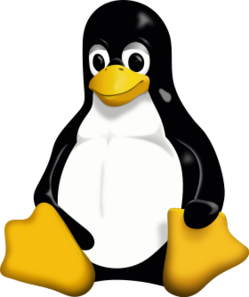
\includegraphics[width=.08\textwidth]{logo-tux.png}\hfill
  
\includegraphics[width=.3\textwidth]{logo-unab.png}\hfill
  
\includegraphics[width=.08\textwidth]{logo-python.png}
}

\makeatletter
\setbeamertemplate{title page}{
  \begin{minipage}[b][\paperheight]{\textwidth}
    \vfill%
    \ifx\inserttitle\@empty\else\usebeamertemplate*{title}\fi
    \ifx\insertsubtitle\@empty\else\usebeamertemplate*{subtitle}\fi
    \usebeamertemplate*{title separator}
    \ifx\beamer@shortauthor\@empty\else\usebeamertemplate*{author}\fi
    \ifx\insertdate\@empty\else\usebeamertemplate*{date}\fi
    \ifx\insertinstitute\@empty\else\usebeamertemplate*{institute}\fi
    \vfill
    \ifx\inserttitlegraphic\@empty\else\inserttitlegraphic\fi
    \vspace*{1cm}
  \end{minipage}
}
\makeatother


\makeatletter
\setlength{\metropolis@titleseparator@linewidth}{2pt}
\setlength{\metropolis@progressonsectionpage@linewidth}{2pt}
\setlength{\metropolis@progressinheadfoot@linewidth}{2pt}
\makeatother


\begin{document}

% ------------------------------------------------------------------------
% Portada de la Presentación
% ------------------------------------------------------------------------
\myfront{}

% ------------------------------------------------------------------------
% Slide 1: Título de la Sesión
% ------------------------------------------------------------------------
\begin{frame}
  \titlepage
  % Ejemplo de título: 
  % \title{Semana 2 - Sesión 2 (Sesión 4): Aplicación de Conceptos Básicos de Python}
\end{frame}

% ------------------------------------------------------------------------
% Slide 2: Índice / Tabla de Contenidos
% ------------------------------------------------------------------------
\begin{frame}
  \frametitle{Resumen - Semana 2, Sesión 2 (Sesión 4)}
  \tableofcontents
\end{frame}

% ------------------------------------------------------------------------
% Configuración de bloques (en caso de usar metrópolis u otro tema)
% ------------------------------------------------------------------------
\metroset{block=fill}

% ----------------------------------------------------------------------------------------
% SECCIÓN 1: Conexión con la Sesión Anterior
% ----------------------------------------------------------------------------------------
\section{Introducción y Repaso}

% ------------------------------------------------------------------------
% Slide 3: Repaso de la Sesión Previa
% ------------------------------------------------------------------------
\begin{frame}{Repaso de la Sesión Previa}
  \begin{itemize}
    \item \textbf{Semana 2, Sesión 1 (Sesión 3)} se centró en:
      \begin{itemize}
        \item Sintaxis básica de Python (indentación, palabras reservadas, comentarios).
        \item Reforzar tipos de datos y operaciones (prioridades, conversión, etc.).
        \item Ejemplos interactivos en Google Colab.
        \item Actividad grupal: \textit{Mini-calculadora}.
      \end{itemize}
    \item \textbf{Objetivo de hoy}: Aplicar estos conceptos en problemas un poco más elaborados.
  \end{itemize}
\end{frame}

% ------------------------------------------------------------------------
% Slide 4: Objetivos de la Sesión 4
% ------------------------------------------------------------------------
\begin{frame}{Objetivos de la Sesión 4}
  \begin{itemize}
    \item \textbf{Consolidar} el manejo de variables, operaciones y sintaxis en Python.
    \item \textbf{Ejercitar} la resolución de problemas más complejos y colaborativos.
    \item \textbf{Fomentar} el razonamiento algorítmico (secuencia, condición, repetición).
    \item \textbf{Preparar} el terreno para estructuras de control (\texttt{if}, \texttt{while}, etc.).
  \end{itemize}
\end{frame}

% ----------------------------------------------------------------------------------------
% SECCIÓN 2: Revisión de Conceptos Clave
% ----------------------------------------------------------------------------------------
\section{Revisión de Conceptos Clave}

% ------------------------------------------------------------------------
% Slide 5: Variables y Operaciones
% ------------------------------------------------------------------------
\begin{frame}{Variables y Operaciones: Recordatorio}
  \begin{itemize}
    \item Las variables se crean con una asignación: \texttt{x = 10}.
    \item \textbf{Operaciones}:
      \begin{itemize}
        \item Suma, resta, multiplicación, división, división entera, exponente.
        \item Uso de paréntesis para priorizar operaciones.
      \end{itemize}
    \item Python es \textbf{dinámico} en tipos: \texttt{x = 3} (int), luego \texttt{x = 3.14} (float).
    \item \textbf{Comentarios} ayudan a documentar el código (\texttt{\#}, \texttt{"""..."""}).
  \end{itemize}
\end{frame}

% ------------------------------------------------------------------------
% Slide 6: Manejo de Entrada/Salida
% ------------------------------------------------------------------------
\begin{frame}[fragile]{Entrada y Salida}
\begin{minted}{python}
user_input = input("Dame un número: ")  # str
num = float(user_input)                 # convierto a float
print(f'Tu número + 10 es: {num + 10}')
\end{minted}
\begin{itemize}
  \item \texttt{input()} siempre regresa una cadena (\texttt{str}).
  \item Para obtener números, se hace \texttt{int()} o \texttt{float()}.
  \item \textbf{Sugerencia}: Manejar excepciones (ej.: \texttt{ValueError}) en casos avanzados.
\end{itemize}
\end{frame}

% ------------------------------------------------------------------------
% Slide 7: Indentación en Python
% ------------------------------------------------------------------------
\begin{frame}{Recordatorio: Indentación}
  \begin{itemize}
    \item \textbf{Bloques} de código definidos por sangría (generalmente 4 espacios).
    \item Usar dos puntos (\texttt{:}) tras \texttt{if}, \texttt{for}, \texttt{while}, etc.
    \item \textbf{Ejemplo simple}:
    \[
      \begin{array}{l}
      \texttt{if x > 0:} \\
      \quad \texttt{print("x es positivo")} \\
      \end{array}
    \]
    \item \textbf{Cuidado}: Mezclar tabulaciones y espacios puede causar errores.
  \end{itemize}
\end{frame}

% ----------------------------------------------------------------------------------------
% SECCIÓN 3: Aplicación de Conceptos
% ----------------------------------------------------------------------------------------
\section{Aplicación de Conceptos}

% ------------------------------------------------------------------------
% Slide 8: Actividad Central
% ------------------------------------------------------------------------
\begin{frame}{Actividad Central: Problemas Paso a Paso}
  \begin{itemize}
    \item Realizaremos 2-3 \textbf{problemas guiados} de dificultad gradual.
    \item Objetivo: Integrar variables, operaciones y lógica básica.
    \item Cada ejercicio se abordará primero en \textbf{colaboración} y luego se compartirá la solución.
  \end{itemize}
\end{frame}

% ------------------------------------------------------------------------
% Slide 9: Ejercicio 1 - Ecuación de Movimiento
% ------------------------------------------------------------------------
\begin{frame}{Ejercicio 1: Ecuación de Movimiento en 1D}
  \begin{block}{Enunciado}
    \begin{itemize}
      \item Dados:
        \begin{itemize}
          \item \texttt{x0}: posición inicial (\(m\)).
          \item \texttt{v0}: velocidad inicial (\(m/s\)).
          \item \texttt{a}: aceleración constante (\(m/s^2\)).
        \end{itemize}
      \item Calcular la posición \(\texttt{x}(t)\) en un tiempo \(\texttt{t}\) usando:
        \[
          x(t) = x0 + v0\cdot t + \frac{1}{2} a t^2
        \]
    \end{itemize}
  \end{block}
  \textbf{Tips}:
  \begin{itemize}
    \item Pedir los datos al usuario.
    \item Imprimir la respuesta con un mensaje que indique la unidad (por ej. metros).
  \end{itemize}
\end{frame}

% ------------------------------------------------------------------------
% Slide 10: Ejercicio 2 - Promedio y Varianza
% ------------------------------------------------------------------------
\begin{frame}{Ejercicio 2: Promedio y Varianza (Intro)}
  \begin{block}{Enunciado}
    \begin{itemize}
      \item Pedir al usuario \textbf{3 valores} (pueden representar mediciones físicas).
      \item Calcular el \textbf{promedio} (\(\bar{x}\)) y la \textbf{varianza} muestral.
      \item Fórmula varianza (para 3 datos):
      \[
        \sigma^2 = \frac{\sum_{i=1}^{3}(x_i - \bar{x})^2}{3 - 1}
      \]
      \item Mostrar ambos resultados.
    \end{itemize}
  \end{block}
  \textbf{Discusión}: Manejo de potencias y restas, y cuidado con divisiones.
\end{frame}

% ------------------------------------------------------------------------
% Slide 11: Ejercicio 3 - Factor de Conversión
% ------------------------------------------------------------------------
\begin{frame}{Ejercicio 3: Factor de Conversión}
  \begin{block}{Enunciado}
    \begin{itemize}
      \item Crear un programa que solicite:
        \begin{itemize}
          \item Un valor numérico (\texttt{valor}).
          \item Una unidad origen (por ej. \texttt{"cm"}, \texttt{"m"}, \texttt{"km"}).
          \item Una unidad destino (\texttt{"cm"}, \texttt{"m"}, \texttt{"km"}).
        \end{itemize}
      \item Convertir \texttt{valor} de la unidad origen a la unidad destino.
      \item Imprimir el resultado final.
    \end{itemize}
  \end{block}
  \textbf{Idea}: Reutilizar factores como: \(\texttt{1 m} = 100 \texttt{ cm}\), \(\texttt{1 km} = 1000 \texttt{ m}\), etc.
\end{frame}

% ------------------------------------------------------------------------
% Slide 12: Trabajo en Equipo
% ------------------------------------------------------------------------
\begin{frame}{Organización de Equipos de Trabajo}
  \begin{itemize}
    \item Formar \textbf{grupos de 2-3 estudiantes}.
    \item Seleccionar 1-2 ejercicios propuestos (o intentar todos).
    \item Editar un \textbf{notebook compartido} en Google Colab.
    \item \textbf{Objetivo}: Discutir soluciones, anotar dudas y resolver en conjunto.
  \end{itemize}
\end{frame}

% ------------------------------------------------------------------------
% Slide 13: Discusión y Retroalimentación
% ------------------------------------------------------------------------
\begin{frame}{Discusión y Retroalimentación}
  \begin{itemize}
    \item ¿Cuál de los ejercicios fue el más complejo?
    \item ¿En qué parte surgieron errores recurrentes?
    \item ¿Cómo podría hacerse un \textbf{diseño modular} (dividir el problema en funciones)?
  \end{itemize}
  \vspace{0.2cm}
  \textbf{Comparte tus experiencias con la clase.}
\end{frame}

% ------------------------------------------------------------------------
% Slide 14: Posible Solución - Ejercicio 1 (Movimiento)
% ------------------------------------------------------------------------
\begin{frame}[fragile]{Solución Propuesta: Ecuación de Movimiento 1D}
\begin{minted}{python}
x0_str = input("x0 (m): ")
v0_str = input("v0 (m/s): ")
a_str  = input("a  (m/s^2): ")
t_str  = input("t  (s): ")

x0 = float(x0_str)
v0 = float(v0_str)
a  = float(a_str)
t  = float(t_str)

x_t = x0 + v0*t + 0.5*a*(t**2)

print(f'La posición en el tiempo t es: {x_t} m')
\end{minted}
\end{frame}

% ------------------------------------------------------------------------
% Slide 15: Posible Solución - Ejercicio 2 (Promedio/Varianza)
% ------------------------------------------------------------------------
\begin{frame}[fragile]{Solución Propuesta: Promedio y Varianza}
\begin{minted}{python}
vals = []
for i in range(1, 4):
    val_str = input(f"Ingrese valor {i}: ")
    val = float(val_str)
    vals.append(val)

# Promedio
mean = sum(vals) / 3

# Varianza muestral (n=3)
var = 0
for v in vals:
    var += (v - mean)**2
var = var / (3 - 1)

print(f'Promedio = {mean}')
print(f'Varianza = {var}')
\end{minted}
\end{frame}

% ------------------------------------------------------------------------
% Slide 16: Posible Solución - Ejercicio 3 (Conversión)
% ------------------------------------------------------------------------
\begin{frame}[fragile]{Solución Propuesta: Conversión de Unidades}
\begin{minted}{python}
valor_str = input("Valor: ")
unidad_origen = input("Unidad origen (cm, m, km): ")
unidad_destino = input("Unidad destino (cm, m, km): ")

valor = float(valor_str)
# Convertir primero a metros
if unidad_origen == "cm":
    valor_m = valor / 100.0
elif unidad_origen == "m":
    valor_m = valor
elif unidad_origen == "km":
    valor_m = valor * 1000
else:
    valor_m = None
# Convertir metros a destino
if unidad_destino == "cm":
    result = valor_m * 100.0
elif unidad_destino == "m":
    result = valor_m
elif unidad_destino == "km":
    result = valor_m / 1000
else:
    result = None

print(f'Resultado: {result} {unidad_destino}')
\end{minted}
\end{frame}

% ------------------------------------------------------------------------
% Slide 17: Análisis de Soluciones
% ------------------------------------------------------------------------
\begin{frame}{Análisis de las Soluciones}
  \begin{itemize}
    \item \textbf{For Loops} y \texttt{range}: usados en Ej. 2 para leer múltiples valores.
    \item \textbf{if/elif/else} (Ej. 3): Estructura para manejar casos y evitar errores de usuario.
    \item \textbf{Validaciones}: No cubrimos todas, pero en casos avanzados se revisan entradas inválidas.
    \item \textbf{Reutilización de código}: Cómo podríamos organizarlo en funciones (tema futuro).
  \end{itemize}
\end{frame}

\section{Ejercicio a Evaluar // Tarea Semanal}
% ------------------------------------------------------------------------
% Slide 18: Ejercicio Adicional (Desafío)
% ------------------------------------------------------------------------
\begin{frame}{Ejercicio a Evaluar}
  \begin{block}{Calculadora Físico-Química}
    \begin{itemize}
      \item Pedir al usuario que seleccione:
        \begin{itemize}
          \item (1) Calcular densidad (\(\rho = \frac{m}{V}\))
          \item (2) Calcular fuerza (\(F = m \cdot a\))
          \item (3) Calcular energía cinética (\(E_c = \frac{1}{2}mv^2\))
        \end{itemize}
      \item Con base en la elección, se piden los datos correspondientes y se muestra el resultado.
      \item Se puede repetir o terminar el programa tras cada operación.
    \end{itemize}
  \end{block}
\end{frame}

% ------------------------------------------------------------------------
% Slide 19: Práctica Individual / Exposición
% ------------------------------------------------------------------------
%\begin{frame}{Práctica Individual}
%  \begin{itemize}
%    \item Si terminaste los ejercicios previos, intenta implementar el “Calculadora Físico-Química”.
%    \item Comenta tu código para cada sección (explica qué pides y por qué).
%    \item \textbf{Opcional}: Usa un \texttt{while} para permitir múltiples operaciones en una sola ejecución.
%  \end{itemize}
%\end{frame}

% ------------------------------------------------------------------------
% Slide 20: Retroalimentación Colectiva
% ------------------------------------------------------------------------
\begin{frame}{Retroalimentación Colectiva}
  \begin{itemize}
    \item ¿Alguno de los ejercicios resultó especialmente difícil?
    \item ¿Cómo han manejado los \textbf{mensajes de error} (entradas inválidas)?
    \item \textbf{Sugerencia}: Documentar mejor tus funciones para cuando construyamos proyectos más grandes.
  \end{itemize}
  \begin{block}{Recuerden}
    El grupo debe entregar el resultado en la plataforma CANVAS
  \end{block}
\end{frame}

% ----------------------------------------------------------------------------------------
% SECCIÓN 4: Conclusiones y Próximos Pasos
% ----------------------------------------------------------------------------------------
\section{Conclusiones}

% ------------------------------------------------------------------------
% Slide 21: Síntesis de la Sesión
% ------------------------------------------------------------------------
\begin{frame}{Síntesis de la Sesión 4}
  \begin{itemize}
    \item Ampliamos ejercicios que involucran:
      \begin{itemize}
        \item Operaciones matemáticas en escenarios reales (movimiento, varianza, conversiones).
        \item Manejo de datos desde el usuario.
        \item Estructuración básica (\texttt{if}, \texttt{for}) sin profundizar en la teoría de control (eso vendrá pronto).
      \end{itemize}
    \item Vimos la importancia de la \textbf{colaboración} y la \textbf{discusión} para resolver problemas.
  \end{itemize}
\end{frame}

% ------------------------------------------------------------------------
% Slide 22: Preparación para Estructuras de Control
% ------------------------------------------------------------------------
\begin{frame}{Preparación para Estructuras de Control}
  \begin{itemize}
    \item Próximamente: \textbf{Unidad III} del Syllabus (Controladores \texttt{if}, \texttt{while}, \texttt{break}, \texttt{continue}, etc.).
    \item \textbf{Recomendación}:
      \begin{itemize}
        \item Revisar cómo usar \texttt{while} para repeticiones indefinidas.
        \item Entender la diferencia entre \texttt{while} y \texttt{for}.
      \end{itemize}
    \item \textbf{Recordar}: Python 3.x es la versión recomendada. Fíjate en \texttt{/} vs \texttt{//}.
  \end{itemize}
\end{frame}

% ------------------------------------------------------------------------
% Slide 23: Recursos y Lecturas
% ------------------------------------------------------------------------
\begin{frame}{Recursos y Lecturas}
  \begin{itemize}
    \item \href{https://docs.python.org/3/tutorial/controlflow.html}{\textbf{Python Docs - Control Flow}} (para un vistazo previo).
    \item \href{https://www.learnpython.org/}{\textbf{LearnPython.org}} (ejercicios básicos).
    \item \href{https://realpython.com/python-basics/}{\textbf{Real Python - Python Basics}} (material de repaso).
  \end{itemize}
\end{frame}

% ------------------------------------------------------------------------
% Slide 24: Consejos de Autoaprendizaje
% ------------------------------------------------------------------------
\begin{frame}{Consejos de Autoaprendizaje}
  \begin{itemize}
    \item \textbf{Practicar todos los días}: sesiones cortas pero frecuentes.
    \item \textbf{Explorar ejemplos reales}: si te gusta la astronomía, intenta con datos de planetas o estrellas.
    \item \textbf{Comentar y Documentar} tu código: te ayudará a recordar qué hiciste la próxima vez.
  \end{itemize}
\end{frame}

% ------------------------------------------------------------------------
% Slide 25: Cierre de Sesión
% ------------------------------------------------------------------------
\begin{frame}
  \Huge{\centerline{¡Muchas gracias!}}
  \vspace{0.3cm}
  \normalsize
  \begin{itemize}
    \item Recuerda guardar tu trabajo en Google Drive.
    \item La próxima sesión profundizaremos en \texttt{if}, \texttt{while} y estructuras de control.
    \item ¡Sigan practicando con los ejercicios adicionales!
  \end{itemize}
\end{frame}

\end{document}

